\documentclass[a4paper,10pt]{article}

% ---------- Fonts and page layout ----------
% （注）フォント名は本環境（macOS + Tectonic）で解決できる表記に合わせ，
%  phase2 レポートの TeXGyreTermes / TeXGyreHeros をスペース入り正式名で指定している。
\usepackage{xeCJK}
\setmainfont{TeX Gyre Termes}
\setsansfont{TeX Gyre Heros}
\setmonofont{DejaVu Sans Mono}
\setCJKmainfont{Noto Serif CJK JP}
\setCJKsansfont{Noto Sans CJK JP}
\setCJKmonofont{Noto Sans Mono CJK JP}
\XeTeXlinebreaklocale "ja"
\XeTeXlinebreakskip=0pt plus 1pt

\usepackage[a4paper,left=24mm,right=24mm,top=24mm,bottom=25mm]{geometry}
\usepackage{setspace}
\setstretch{1.15}
\setlength{\parindent}{1em}
\setlength{\parskip}{0.25em}

% ---------- Math, tables, figures ----------
\usepackage{amsmath,amssymb,mathtools}
\usepackage{graphicx}
\usepackage{booktabs}
\usepackage{longtable}
\usepackage{tabularx}
\usepackage{array}
\usepackage{multirow}
\usepackage{makecell}
\usepackage{float}
\usepackage{caption}
\usepackage{xcolor}
\usepackage{enumitem}
\usepackage{titlesec}
\usepackage{fancyhdr}
\usepackage[hidelinks]{hyperref}
\usepackage{url}
\usepackage{microtype}
\usepackage[most]{tcolorbox}

\graphicspath{{figures/}}

% ---------- Unified style ----------
\definecolor{bbblack}{HTML}{222222}
\definecolor{bbgray}{HTML}{666666}
\definecolor{bblight}{HTML}{F2F2F2}
\definecolor{bbline}{HTML}{333333}
\renewcommand{\figurename}{Figure}
\renewcommand{\tablename}{Table}
\captionsetup{font={small},labelfont={bf},justification=raggedright,singlelinecheck=false}
\captionsetup[table]{position=top}
\captionsetup[figure]{position=bottom}
\renewcommand{\arraystretch}{1.22}
\setlist[itemize]{leftmargin=1.6em,itemsep=0.15em,topsep=0.2em}
\setlist[enumerate]{leftmargin=1.8em,itemsep=0.15em,topsep=0.2em}

\titleformat{\section}{\sffamily\bfseries\Large\color{bbblack}}{\thesection}{0.8em}{}
\titleformat{\subsection}{\sffamily\bfseries\large\color{bbblack}}{\thesubsection}{0.7em}{}
\titleformat{\subsubsection}{\sffamily\bfseries\normalsize\color{bbblack}}{\thesubsubsection}{0.6em}{}
\titlespacing*{\section}{0pt}{1.2em}{0.5em}
\titlespacing*{\subsection}{0pt}{0.9em}{0.35em}
\titlespacing*{\subsubsection}{0pt}{0.7em}{0.25em}

\pagestyle{fancy}
\fancyhf{}
\lhead{\small\sffamily BEYOND BUFFETT Phase5 Methodology}
\rhead{\small\sffamily 検証：in-sampleのリスク確認}
\cfoot{\small\thepage}
\renewcommand{\headrulewidth}{0.4pt}

\newcolumntype{Y}{>{\raggedright\arraybackslash}X}
\newcommand{\metric}[1]{\mathrm{#1}}
\newcommand{\ind}[1]{\mathbf{1}\{#1\}}

\newtcolorbox{keybox}[1][]{
  colback=bblight, colframe=bblight, boxrule=0pt, arc=1mm,
  left=2mm, right=2mm, top=2mm, bottom=2mm, breakable,
  before skip=6pt, after skip=6pt,
  title={#1}, coltitle=bbblack, fonttitle=\sffamily\bfseries,
  attach title to upper={\par}
}
\newtcolorbox{defbox}[1][直感]{
  colback=white, colframe=bbline, boxrule=0.6pt, arc=1mm,
  left=2mm, right=2mm, top=2mm, bottom=2mm, breakable,
  before skip=6pt, after skip=6pt,
  title={#1}, coltitle=bbblack, fonttitle=\sffamily\bfseries,
  attach title to upper={\par}
}

\begin{document}

% ---------- Cover ----------
\begin{titlepage}
\centering
\vspace*{12mm}
{\sffamily\bfseries\Huge BEYOND BUFFETT\par}
\vspace{6mm}
{\sffamily\bfseries\LARGE Phase5 解説レポート\par}
\vspace{3mm}
{\sffamily\Large 検証：成績を誇るのではなく，壊れにくさを確かめる\par}
\vspace{14mm}
{\large 本資料は，最終 20 社と配分に対して行った標本内（in-sample）の\par}
{\large リスク特性確認と，16 通りのアブレーション（分解検査）を，\par}
{\large 「何が言えて，何が言えないか」まで含めて 0 から解説する。\par}
\vfill
{\small 正典データ：phase5\_verification\_and\_ablation/phase5\_validation\_summary.json\par}
\end{titlepage}

\setcounter{tocdepth}{2}
\tableofcontents
\clearpage

% ---------- 1 ----------
\section{エグゼクティブサマリー}

Phase5 の目的は，このポートフォリオが儲かることの証明ではない。構築に使ったのと同じ期間で成績を測っても，それは未来の証明にならない。私たちが確かめたのは，（i）過去データ上のリスクの姿（値動き・下落・市場連動），（ii）リターンがどの役割・テーマに依存していたか，（iii）選定がどの設計判断に依存しているか（アブレーション），の三点である。

\begin{keybox}[Phase5 の一文定義]
\centering
\Large 成績を誇るのではなく，壊れにくさと依存構造を確かめる。
\end{keybox}

主要な結果は次の通りである。3 年（標本内）で年率リターン $+30.8\%$（TOPIX $+24.1\%$），年率ボラティリティ $21.9\%$，最大ドローダウン $-24.9\%$（TOPIX $-23.3\%$），ベータ $0.925$，Sharpe $1.41$，Jensen's $\alpha$ $+7.3\%$/年。\textbf{一方，直近 1 年の Information Ratio は $-0.405$（負）であり，市場に負けている。}この事実を隠さないことが，本研究の立場（性能を主張しない）の直接の根拠である。アブレーションでは，候補宇宙を Top100 に狭めた場合（A8）に一致が 7 社まで落ち，「破で候補を 1{,}200 社へ広げた判断」が選定の背骨であることが分かった。

\section{この資料の読み方}

\ref{sec:insample}節で標本内（in-sample）という概念を 0 から定義する。ここを飛ばすと，本資料のすべての数値を誤読する。\ref{sec:data}節でデータと補正，\ref{sec:risk}節でリスク指標，\ref{sec:contrib}節で寄与分解と除外変種，\ref{sec:ablation}節でアブレーション，\ref{sec:risks}節でリスク一覧，\ref{sec:limits}節で限界を読む。

% ---------- 2 ----------
\section{in-sample（標本内）を0から理解する}
\label{sec:insample}

\begin{keybox}[フローでの位置]
本資料のすべての成績系数値には「標本内」という限定がつく。銘柄選定にはどの検証式も使っていない。検証で良かったから銘柄や比率を変える，という後知恵は一度も行っていない。
\end{keybox}

本ポートフォリオは 2026 年 6 月時点で入手可能なデータから構築した。その 20 社の過去 3 年の成績を測ると，測定期間は構築に使った情報の期間と重なる。これが標本内（in-sample）である。標本内の好成績は「過去に良かった銘柄を選べば過去の成績が良い」という同語反復に近づくため，将来の成果の証明にはならない（Bailey et al., 2014；López de Prado, 2018）。

\begin{defbox}
たとえば，過去 3 年で最も上がった 20 銘柄を今日選び，その 3 年成績を測れば必ず素晴らしい数字が出る。それは予測力ではない。本研究の選定は成績で選んでいないため，この最悪の形は避けているが，それでも構築時点の情報と測定期間が重なる以上，標本内の限定は消えない。だから私たちは，リターンの高さではなく，リスクの姿と依存構造だけを主張する。
\end{defbox}

生存者バイアス（上場廃止銘柄が母集団から欠けること）や先読みバイアス（開示前の情報を使ってしまうこと）の可能性も残る。Phase2 の point-in-time パネルで部分的に対処したが，完全ではない。

% ---------- 3 ----------
\section{データと修理：ベンチマークの分割補正}
\label{sec:data}

価格は日次の調整済み終値（2021-06〜2026-06，約 3{,}650 銘柄）を用い，ベンチマークは TOPIX 連動 ETF（1306.T）と日経平均（\^{}N225）とした。検証コードは，1306.T の原系列に未調整の 1 対 10 株式分割（2026-03-30）が混入し同日に約 $-90\%$ の不連続が生じることを検出したため，同日以降の価格を 10 倍して連続化した。ポートフォリオ構成銘柄には分割様の不連続はなく，塩水港精糖（2112）の 2024-01-25 の $+32.9\%$ は実際の値動きとして保持した。データの掃除も検証の一部である。

% ---------- 4 ----------
\section{リスク指標を0から理解する}
\label{sec:risk}

\subsection{値動きの大きさ：ボラティリティ}

日々の収益率のばらつき（標準偏差）を年率換算した値である。本ポートフォリオは 3 年で $21.9\%$。数字単体に良し悪しはなく，市場（TOPIX）と比べて過度でないかを見る。

\subsection{リスクあたりの効率：Sharpe Ratio}

\begin{equation}
\metric{Sharpe} \;=\; \frac{\bar r_p - r_f}{\sigma_p}.
\label{eq:sharpe}
\end{equation}

$\bar r_p$ は年率リターン，$r_f$ は無リスク金利（本研究では約 0），$\sigma_p$ は年率ボラティリティである（Sharpe, 1966; 1994）。3 年で $1.41$——ただし標本内の値である。

\subsection{最悪期の下落：Maximum Drawdown}

\begin{equation}
\metric{MDD} \;=\; \min_{t}\left(\frac{C_t}{\max_{s\le t} C_s}-1\right).
\label{eq:mdd}
\end{equation}

$C_t$ は累積価値である。ピークからの最大下落率で，3 年で $-24.9\%$（TOPIX $-23.3\%$）。市場並みの落ち込みに収まっている。

\subsection{市場で説明できない分：ベータと Jensen's α}

\begin{equation}
\alpha_p \;=\; \bar r_p - \beta_p\,\bar r_m,
\qquad
\beta_p \;=\; \frac{\operatorname{Cov}(r_p, r_m)}{\operatorname{Var}(r_m)}.
\label{eq:alpha}
\end{equation}

$\beta_p=0.925$ は，市場が 1\% 動くとき平均 0.925\% 動く「やや守備的」な連動度を示す。$\alpha_p=+7.3\%$/年は市場変動で説明できない上乗せだが，標本内であり将来の $\alpha$ を約束しない（Jensen, 1968）。

\subsection{市場に勝ち続けたか：Information Ratio}

\begin{equation}
\metric{IR} \;=\; \frac{\bar r_p - \bar r_b}{\sigma_{p-b}}.
\label{eq:ir}
\end{equation}

$\bar r_b$ はベンチマーク，$\sigma_{p-b}$ は超過リターンのぶれ（トラッキングエラー）である。3 年では $+0.445$ だが，\textbf{直近 1 年は $-0.405$ と負}である。期間で符号が変わる——この一点だけでも，超過収益を「実力」と断定できないことが分かる。

\begin{defbox}
1 年 IR が負という事実は，本研究にとって都合が悪い数字である。それでも本文に載せるのは，都合の悪い数字を出せることが，残りの数字の信頼性を支えるからである。私たちがこの 20 社を持てる根拠は成績ではなく，三世代の堀という構造と証拠にある。
\end{defbox}

\begin{table}[H]
\caption{リスク指標の実測値（標本内）}
\centering
\small
\begin{tabular}{lrr}
\toprule
指標 & 3 年 & 1 年 \\
\midrule
年率リターン（ポート／TOPIX） & $+30.8\%$／$+24.1\%$ & $+37.9\%$／$+40.7\%$ \\
年率ボラティリティ & $21.9\%$ & $18.5\%$ \\
最大ドローダウン & $-24.9\%$ & $-11.7\%$ \\
Sharpe（式\eqref{eq:sharpe}） & $1.41$ & $2.04$ \\
$\beta$／$\alpha$（式\eqref{eq:alpha}） & $0.925$／$+7.3\%$ & $0.835$／$+3.6\%$ \\
Information Ratio（式\eqref{eq:ir}） & $+0.445$ & $\mathbf{-0.405}$ \\
\bottomrule
\end{tabular}
\end{table}

\subsection{集中の度合い：HHI}

\begin{equation}
\metric{HHI} \;=\; \sum_{g}\Big(\sum_{i\in g}\omega_i\Big)^{2}.
\label{eq:hhi}
\end{equation}

グループ比率の 2 乗和で，大きいほど集中している。実測は銘柄 $0.053$・業種 $0.123$・テーマ $0.402$。テーマ（AI 基盤系）の集中がやや高く，これはリスクとして開示する。

% ---------- 5 ----------
\section{寄与分解と除外変種：何がリターンを運んだか}
\label{sec:contrib}

\begin{figure}[H]
\centering
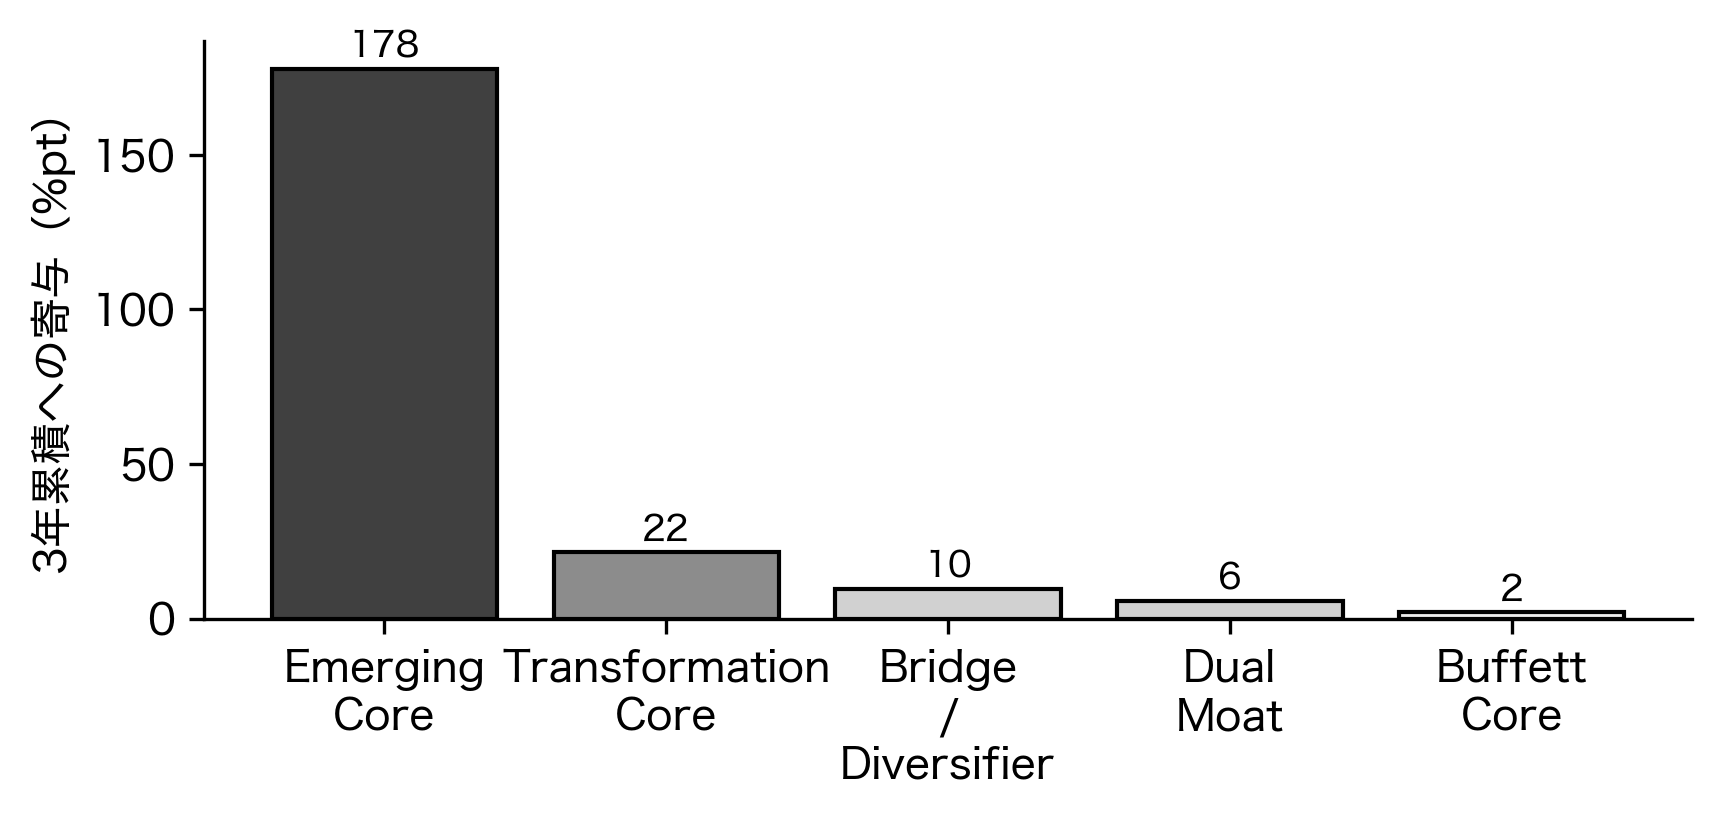
\includegraphics[width=0.8\linewidth]{p5_role_contrib.png}
\caption{役割別の 3 年寄与（\%pt，標本内）。生まれる堀（Emerging Core）が牽引し，完成した堀（Buffett Core）はほぼ土台に徹した。}
\label{fig:contrib}
\end{figure}

役割別では Emerging Core が $+178$\%pt 相当と支配的で，トップ寄与は 5803 フジクラ（光通信）だった。テーマ別でも光通信・半導体が上位である。一社ずつ抜いて測り直す leave-one-out では，どの一社を除いてもボラティリティは $0.210$〜$0.229$ に収まり，リスク構造が単一銘柄に依存していないことを確認した。

除外変種はさらに示唆的である。AI 基盤テーマの 8 社を外すとリターンは約半分（$+17.5\%$）に落ち，ボラは下がる——リターンの源泉もリスクの源泉も Emerging 側にある。逆に低 PBR（変わる堀側）の 12 社を外すとリターンは上がるが，ボラは $35.5\%$，最大下落は $-44.5\%$ へ悪化する——\textbf{割安株は攻めではなく，緩衝材として効いている}。三世代を束ねる設計の意味が，ここに数字で現れている。

% ---------- 6 ----------
\section{アブレーション：設計のどこが効いているのか}
\label{sec:ablation}

\begin{keybox}[フローでの位置]
アブレーション（ablation＝切除）は，設計の条件を一つずつ外して再選定し，最終 20 社と何社一致するかを測る分解検査である。成績は一切使わない。目的は「選定が単一の仕掛け・単一テーマ・後付け調整に依存していないこと」の確認である。
\end{keybox}

検査は A1〜A16 の 16 通り。実行前に，全条件を適用したベースラインが実際の最終 20 社を 20/20 で再現することを確認した（再現しない検査は無意味だからである）。

\begin{figure}[H]
\centering
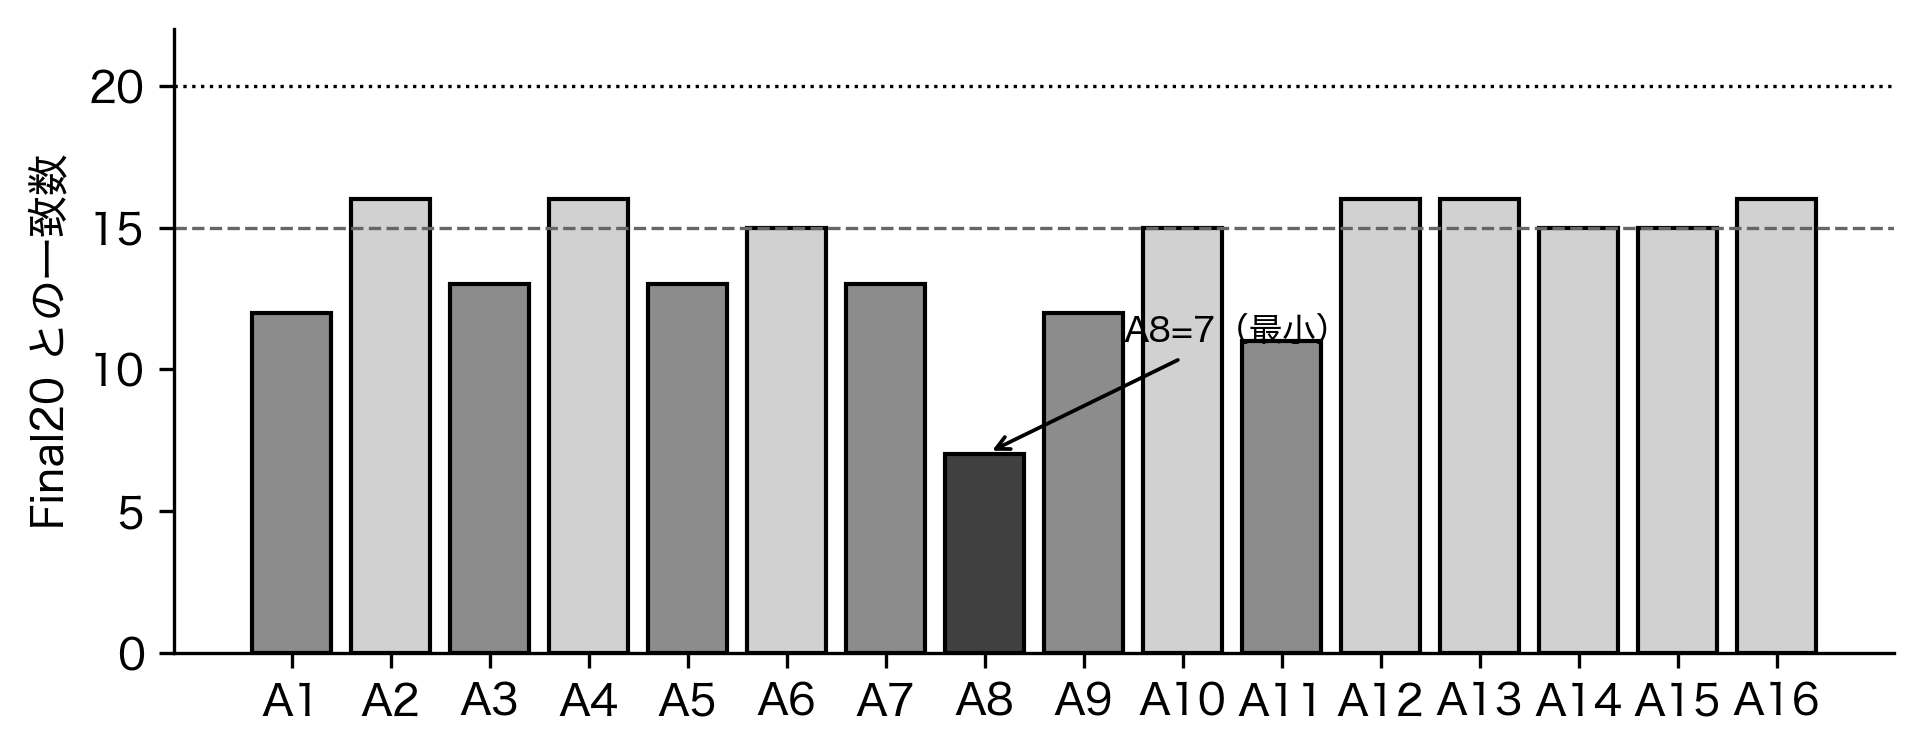
\includegraphics[width=0.95\linewidth]{p5_ablation.png}
\caption{各変種の選定と最終 20 社の一致数。A8（候補を Top100 に限定）が最小の 7。}
\label{fig:ablation}
\end{figure}

読み方は三つある。第一に，最小は A8（Top100 限定，7 社）であり，\textbf{破で候補宇宙を 1{,}200 社へ広げた判断こそが選定の背骨}である。第二に，Transformation のみ（A1，12 社）・Emerging のみ（A2，16 社）はいずれも完全再現に届かず，二軸の合成が本体である。第三に，各種ペナルティや証拠制約を一つ外しても一致は 10 社を下回らない——どの仕掛けも「効いているが，単独で結果を作ってはいない」。なお A16（AI キーワード規制を Emerging 系役割に限定，16 社）は，当該規制が過度に拘束的でないことを示す。

% ---------- 7 ----------
\section{主要なリスク一覧}
\label{sec:risks}

\begin{enumerate}
\item 将来の堀への偏重：寄与が Emerging Core に集中している。
\item AI テーマ過熱：テーマ HHI $0.402$ と高い。剥落時は同時に下がりうる。
\item 変わる堀の割安のワナ：改善が止まれば低評価が固定化する。
\item 開示不足による過小・過大評価：Emerging の Level 2 以上は 14 社の個別精査に依存。
\item 流動性・小型株リスク：売買代金の小さい銘柄を含む。
\item 業種集中：同一業種 3 社上限まで使っている業種がある。
\item 単元株の丸め：実単元（L=100）では 9 社が購入不可。単元未満株が前提。
\item 標本内評価の限界：直近 1 年 IR は負。将来を保証しない。
\item 独自合成式の恣意性：重みは設計値（$\pm20\%$ 感度で選定不変を確認）。
\item データ品質：1306.T の分割補正など，原データの掃除に依存する。
\end{enumerate}

\subsection{ミニ演習：この数字から言ってよいこと}

「3 年 Sharpe 1.41」から言ってよいのは，「過去 3 年・標本内では，リスクの割に効率的だった」までである。「今後も市場に勝てる」は言えない（1 年 IR が負である）。言えることと言えないことの境界を数字ごとに引く——それが Phase5 の目的である。

% ---------- 8 ----------
\section{限界と誠実な書き方}
\label{sec:limits}

\begin{itemize}
\item すべての成績系数値は標本内であり，将来の運用成果を保証しない。
\item 生存者バイアス・先読みバイアスの可能性が残る（point-in-time で部分対処）。
\item アブレーションは構造の類似度を測るもので，リターンの優劣を測るものではない。
\item 除外変種の解釈（緩衝材など）は事後的な観察であり，因果の証明ではない。
\end{itemize}

\subsection{本文で使える要約文}
\begin{keybox}
検証は，将来リターンの証明ではなく，過去データ上のリスク特性と依存構造の確認として行った。3 年（標本内）で年率 $+30.8\%$・ボラ $21.9\%$・最大下落 $-24.9\%$・$\beta\,0.925$ である一方，直近 1 年の Information Ratio は $-0.405$ と負であり，超過収益を主張しない。寄与は生まれる堀（光通信・半導体）に集中し，低 PBR 銘柄を外すとボラが $35.5\%$ へ悪化することから，変わる堀は緩衝材として機能した。16 通りのアブレーションでは，候補宇宙を Top100 に狭めた場合の一致が 7 社と最小で，破の「候補を 1{,}200 社へ広げる」判断が選定の背骨であることを確認した。
\end{keybox}

% ---------- Appendix ----------
\newpage
\section{Appendix A：変数一覧}
\begin{longtable}{p{26mm}p{44mm}p{74mm}}
\caption{Phase5 で使う主な変数}\\
\toprule
記号 & 名称 & 意味 \\
\midrule
\endfirsthead
\toprule
記号 & 名称 & 意味 \\
\midrule
\endhead
$r_p, r_b, r_m$ & 収益率 & ポートフォリオ／ベンチマーク／市場の日次収益率。 \\
$\sigma_p$ & 年率ボラティリティ & 日次収益率の標準偏差の年率換算。 \\
$C_t$ & 累積価値 & 期首を 1 とした累積指数。 \\
$\metric{MDD}$ & 最大ドローダウン & ピーク比の最大下落率（式\eqref{eq:mdd}）。 \\
$\beta_p$ & ベータ & 市場との連動度（式\eqref{eq:alpha}）。 \\
$\alpha_p$ & Jensen's α & 市場で説明できない超過（標本内）。 \\
$\sigma_{p-b}$ & トラッキングエラー & 超過リターンのぶれ。 \\
$\metric{IR}$ & Information Ratio & 超過の安定度（式\eqref{eq:ir}）。1 年は $-0.405$。 \\
$\metric{HHI}$ & 集中度 & 比率の 2 乗和（式\eqref{eq:hhi}）。 \\
A1〜A16 & アブレーション & 条件を外した再選定と Final20 の一致数。 \\
\bottomrule
\end{longtable}

\section{References}
\begin{itemize}
\item Bailey, D. H., Borwein, J., L\'opez de Prado, M., \& Zhu, Q. J. (2014). Pseudo-Mathematics and Financial Charlatanism. \emph{Notices of the AMS}, 61(5), 458--471.
\item Jaccard, P. (1901). \'Etude comparative de la distribution florale. \emph{Bulletin de la Soci\'et\'e Vaudoise des Sciences Naturelles}, 37, 547--579.
\item Jensen, M. C. (1968). The Performance of Mutual Funds in the Period 1945--1964. \emph{Journal of Finance}, 23(2), 389--416.
\item L\'opez de Prado, M. (2018). \emph{Advances in Financial Machine Learning}. Wiley.
\item Sharpe, W. F. (1966). Mutual Fund Performance. \emph{Journal of Business}, 39(1), 119--138.
\item Sharpe, W. F. (1994). The Sharpe Ratio. \emph{Journal of Portfolio Management}, 21(1), 49--58.
\end{itemize}

\end{document}
